\documentclass[10pt,a4paper]{amsart}
\usepackage[margin=19mm]{geometry}
\usepackage{amsmath,amssymb,mathtools}
\usepackage[scr=rsfs,cal=euler]{mathalfa}
\usepackage{xfrac}
\usepackage[unicode,hidelinks,bookmarks=false]{hyperref}
\newcommand{\ie}{i.e.\ }
\newcommand{\cf}{cf.\ }
\newcommand{\resp}{respectively\ }
\newcommand{\Subsection}{\subsection}
\providecommand{\nobreakdash}{\nobreak\hbox{-}}
\setlength{\emergencystretch}{2em}
\multlinegap0pt
\usepackage{tikz}
\usepackage[all]{xy}
\newtheorem{lemma}{Lemma}
\newcommand{\flo}[1]{\left\lfloor\frac{#1}{2}\right\rfloor}
\title{Corrigendum to ``Higher Lorentzian polynomials, higher Hessians, and the Hodge-Riemann relations for graded oriented Artinian Gorenstein algebras in codimension two'', [International Mathematics Research Notices, Volume 2025, Issue 13, July 2025]}
\author{Pedro Macias Marques, Chris McDaniel, Alexandra Seceleanu}
\date{Source: arXiv:2602.09976v1 (CC BY 4.0)}
\begin{document}
\maketitle

\noindent\emph{Source and licence.} Corrigendum to ``Higher Lorentzian polynomials, higher Hessians, and the Hodge-Riemann relations for graded oriented Artinian Gorenstein algebras in codimension two'', [International Mathematics Research Notices, Volume 2025, Issue 13, July 2025]. Version arXiv:2602.09976v1 (CC BY 4.0), distributed by arXiv under the Creative Commons Attribution 4.0 International licence, http://creativecommons.org/licenses/by/4.0/, as recorded in the arXiv licence metadata for this exact version and shown on the abstract page https://arxiv.org/abs/2602.09976v1. Full licence notice: \texttt{licenses/arxiv-2602.09976-CC-BY-4.0.txt}.\par\smallskip

\noindent\textit{Editorial scope.} Counted unit: the article's lemma lem:alpha (source0.tex lines 509--513). The article's complete original proof of it is delivered with it (source0.tex lines 514--653, one \texttt{proof} environment of 140 lines). No mathematics is written, repaired or re-derived: the statement and the proof are the article's own lines, in the article's own notation, and no retained line is substituted or re-flowed.  Retained uncounted as the source-local context the proof needs: lines 363--366; lines 376--381; lines 386--395; lines 483--488; lines 491--494; lines 503--506.  Nothing was omitted from any retained span, so the package carries no omission record.  No retained line contains a citation, so the wrapper carries no bibliography and no bibliography entry.  The retained lines contain the article's own diagram code, which the wrapper typesets with the standard tikz packages; no image file is delivered and the package declares no asset dependency.  Editorial formatting only, in addition: an AMS \texttt{amsart} preamble that restates the article's own declarations and macros used by the retained lines, namely the environments \texttt{lemma} on separate counters, together with the standard packages those lines need.  The retained environments print in this document as Lemma 1 in order of appearance, whereas the article prints the same items with the numbering of its own full document.  The complete native source of the article as distributed in the arXiv e-print for this exact version is bundled unchanged as \texttt{sources/194362/source0.tex}.
\begin{equation}
	\label{eq:nu}
	\nu_{r-q}=(k_q-q)+(r-a), \ \ 0\leq q\leq r.
\end{equation}

\begin{align}
	\label{eq:lambda0}
	\lambda_p= & (j_r-r)+i-(i_p-p), \ 0\leq p\leq r\\
	\label{eq:mu0}
	\mu_q = & (j_r-r)-(j_q-q), \ \ 0\leq q\leq r.
\end{align}

\begin{lemma}
	\label{lem:LRr}
	Fix integers $a,d,i,r$ satisfying $0\leq a<r\leq i\leq \flo{d}$ and assume that $I=\{0\leq i_0<\cdots<i_r\leq i\}$ and $J=\{0\leq j_0<\cdots<j_r\leq d-i\}$ are given with $\lambda$ and $\mu$ defined as in Equation \eqref{eq:lambda0} and Equation \eqref{eq:mu0}.  Then every Littlewood-Richardson partition $\nu=(\nu_0,\ldots,\nu_m)\in\operatorname{LRP}(\lambda/(\mu+a))$ satisfies
	$m=r$ and $\nu_0\leq d-r-a$ and $\nu_r\geq r-a$.  In particular, every $(r+1)\times (r+1)$ minor of $\phi^i_d(F)$ can be written as a nonnegative linear combination of the maximal minors of $\phi^r_d(F)$; explicitly we have,
	\begin{equation}
		\label{eq:DeltaLR}
		\Delta_{IJ}\left(\phi^i_d(F)\right)=\sum_{\nu\in\operatorname{LRP}(\lambda/(\mu+a))}c^{\lambda}_{(\mu+a),\nu}\cdot\Delta_{K(\nu)}\left(\phi^r_d(F)\right)
	\end{equation}
	where $K(\nu)=K=\{0\leq k_0<\cdots<k_r\leq d-r\}$ is defined as in Equation \eqref{eq:nu}.	
\end{lemma}

\begin{align}
	\label{eq:i}
	i_p= & \max\{(i-a)-\nu_p,0\}+p, & 0\leq p\leq r\\
	\label{eq:j}
	j_q= & \max\{\nu_{r-q}-(i-a),0\}+q, & 0\leq q\leq r.
\end{align}

\begin{align}
	\label{eq:K}
	k_q= & \nu_{r-q}-(r-a)+q, & 0\leq q\leq r.
\end{align}

\begin{equation}
	\label{eq:alpha2}
	\alpha^i(\nu)=\sum_{q=t+1}^r\left((i-a)-\nu_q\right).
\end{equation}

\begin{lemma}
	\label{lem:alpha}
	Fix integers $a,d,i,r$ satisfying $0\leq a\leq r\leq i\leq \flo{d}$, and fix $r+1$-subsets $I$, $J$ and $K$ defined by Equations \eqref{eq:i}, \eqref{eq:j}, and \eqref{eq:K} above, with $i\leq k_r\leq d-r$.  Then in the Littlewood-Richardson expansion of the minor $\Delta_{IJ}(\phi^i_d(F))$, as in Lemma \ref{lem:LRr}, the minor $\Delta_K(\phi^r_d(F))$ occurs with Littlewood-Richardson coefficient $1$ and maximal $\alpha^i(K)$, i.e.
	$$\Delta_{IJ}\left(\phi^i_d(F)\right)=\Delta_K\left(\phi^r_d(F)\right)+\sum_{\substack{\nu'\in\operatorname{LRP}(\lambda/(\mu+a))\\ \alpha^i(K')<\alpha^i(K)\\}}c^\lambda_{(\mu+a),\nu'}\cdot \Delta_{K'}\left(\phi^r_d(F)\right).$$
\end{lemma}

\begin{proof}
	For concreteness, let us introduce coordinates for the boxes of the Young diagram of $\lambda/(\mu+a)$ so that the lower left corner is at the origin.  Define the critical line to be the vertical line $x=\lambda_0-(i-a)$.  Our first observation is that for any Littlewood-Richardson tableau $T\in\operatorname{LRT}(\lambda/(\mu+a))$, the reverse lattice word condition as well as the column-strict condition implies that entries of $T$ lying to the right of the critical line are fixed, i.e. the $p^{th}$ row must contain only $p$'s for $0\leq p\leq r$.  Moreover, if $t$, $0\leq t\leq r$ is the largest index for which $\nu_t\geq (i-a)$, then we claim that there is exactly one Littlewood-Richardson tableau $T$ whose entries to the left of the critical line all lie in $\{0,\ldots,t\}$.  To see this, start filling in the boxes to the left of the critical line, column by column moving top to bottom and from right to left.  Note that the righter-most column to the left of the critical line has $t_1=\#\left\{p \ | \ \nu_p\geq (i-a)+1\right\}$ boxes where $t_1\leq t$.  Hence, by the reverse lattice and column-strict properties, the entries in that column must be exactly $\{0,\ldots,t_1-1\}$.  Inductively, the $q^{th}$ righter-most column to the left of the critical line has $t_q=\#\{p \ | \ \nu_p\geq (i-a)+q\}$ boxes where $t_q\leq t_{q-1}\leq \cdots\leq t_1\leq t$.  Moreover the entries in those boxes can only be $\{0,\ldots,t_{q-1}-1\}$ by the weakly increasing row property.  Again by the reverse lattice word property, it follows that the boxes in the $q^{th}$ righter-most column to the left of the critical line must be filled with the numbers $\{0,\ldots,t_q-1\}$.  This shows that the entries of $T\in\operatorname{LRT}_\nu(\lambda/(\mu+a))$ are uniquely determined, and hence $c^\lambda_{(\mu+a),\nu}=1$.
	
	
	Finally, if $\nu'$ is any other Littlewood-Richardson partition for $\lambda/(\mu+a)$ distinct from $\nu$, then it must differ in the entries $\{t+1,\ldots,r\}$ and hence we must have $\nu'_j\geq \nu_j$ for each $j\in\{t+1,\ldots,r\}$ with strict inequality for at least one $j$.  Therefore, it follows from Equation \eqref{eq:alpha2} that we must have $\alpha^i(K')=\alpha^i(\nu')<\alpha^i(\nu)=\alpha^i(K)$, and the second statement follows from Lemma \ref{lem:LRr}.
	%Then the Littlewood-Richardson condition implies that in any Littlewood-Richardson tableau $T'$ corresponding to $\nu'$, its entries to the right of the vertical line $x=\nu_0-(i-a)$ must be the same as that of $\nu$, namely the $k^{th}$ row must consist of only $k$'s to the right of that line.  Let $t$, $0\leq t\leq r$ be the largest index for which $\nu_t-(i-a)\geq 0$.  Then we further observe that for any Littlewood-Richardson filling of the Young diagram of $\lambda/(\mu+a)$, if the entries in the boxes that lie to the left of the line $x=d-r-(i-a)$ use only the numbers $\{0,\ldots,t\}$, then that filling is unique and its content must be $\nu$, again by the Littlewood-Richardson condition.  Therefore if $\nu'$ and $\nu$ are different, they must differ by their entries in $\{t+1,\ldots,r\}$.  On the other hand, if $\nu'$ has numbers from $\{t+1,\ldots,r\}$ to the left of the line $x=d-r-(i-a)$ then its $\alpha^i$-statistic must be strictly smaller than that of $\nu$, since the numbers in $\{t+1,\ldots,r\}$ only occur to the right of the line $x=d-r-(i-a)$ in the filling corresponding to $\nu$.  
	See Figure \ref{fig:LambdaMu}.
	
	
	
	
	
	\begin{figure}
		\begin{center}
			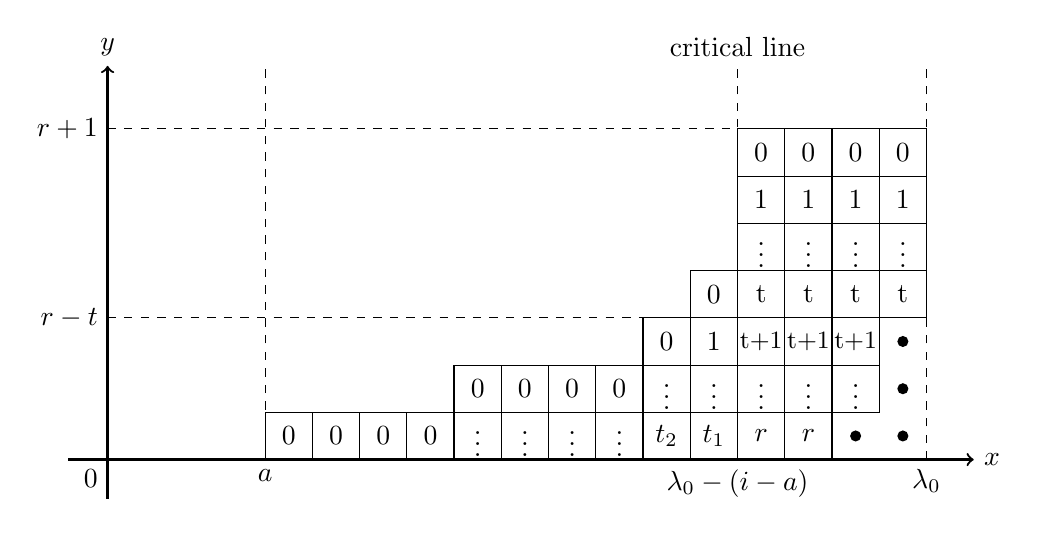
\begin{tikzpicture}[scale=1]
				% Axes
				\draw[->, thick] (-0.5,0) -- (11,0) node[right] {$x$};
				\draw[->, thick] (0,-0.5) -- (0,5) node[above] {$y$};
				% Origin
				\node[below left] at (0,0) {$0$};
				% X-axis points
				\coordinate (a) at (2,0);
				\coordinate (b) at (8,0);
				\coordinate (lam) at (10.4,0);
								
				\node[below] at (a) {$a$};
				\node[below] at (lam) {$\lambda_0$};
				\node[below] at (b) {$\lambda_0-(i-a)$};
				
				% Y-axis points
				\coordinate (rp1) at (0,1.8);
				\coordinate (rmt) at (0,4.2);
				
				\node[left] at (rp1) {$r-t$};
				\node[left] at (rmt) {$r+1$};
				
				\node[above] at (8,5) {critical line};
				
				% Dashed vertical lines (first quadrant only)
				\draw[dashed] (2,0) -- (2,5);
				\draw[dashed] (8,0) -- (8,5);
				\draw[dashed] (10.4,0) -- (10.4,5);
				
				
				% Dashed horizontal lines (first quadrant only)
				\draw[dashed] (0,1.8) -- (8,1.8);
				\draw[dashed] (0,4.2) -- (8,4.2);
				
				% ---- BOX STRIP ABOVE X-AXIS ----
				\def\boxsize{0.6}
				\def\ybox{0} % vertical offset above x-axis
				
				% Starting x at point a
				\def\xstart{2}
				
				% First 4 boxes labeled 0
				\foreach \i in {0,...,3} {
					\draw (\xstart+\i*\boxsize, \ybox)
					rectangle ++(\boxsize,\boxsize);
					\node at (\xstart+\i*\boxsize+0.5*\boxsize, \ybox+0.5*\boxsize) {$0$};
				}
				\foreach \i in {4,...,7} {
					\draw (\xstart+\i*\boxsize, \ybox+\boxsize)
					rectangle ++(\boxsize,\boxsize);
					\node at (\xstart+\i*\boxsize+0.5*\boxsize, \ybox+1.5*\boxsize) {$0$};
				}
				
				\foreach \i in {10,...,13} {
					\draw (\xstart+\i*\boxsize, \ybox+6*\boxsize)
					rectangle ++(\boxsize,\boxsize);
					\node at (\xstart+\i*\boxsize+0.5*\boxsize, \ybox+6.5*\boxsize) {$0$};
				}
				
				% Next 4 boxes labeled 1
				
				\foreach \i in {10,...,13} {
					\draw (\xstart+\i*\boxsize, \ybox+5*\boxsize)
					rectangle ++(\boxsize,\boxsize);
					\node at (\xstart+\i*\boxsize+0.5*\boxsize, \ybox+5.5*\boxsize) {$1$};
				}
				
				% Next 4 boxes labeled \vdots
				\foreach \i in {4,...,7} {
					\draw (\xstart+\i*\boxsize, \ybox)
					rectangle ++(\boxsize,\boxsize);
					\node at (\xstart+\i*\boxsize+0.5*\boxsize, \ybox+0.5*\boxsize) {$\vdots$};
				}
				
				\foreach \i in {8,...,12} {
					\draw (\xstart+\i*\boxsize, \ybox+\boxsize)
					rectangle ++(\boxsize,\boxsize);
					\node at (\xstart+\i*\boxsize+0.5*\boxsize, \ybox+1.5*\boxsize) {$\vdots$};
				}
				
				\foreach \i in {10,...,13} {
					\draw (\xstart+\i*\boxsize, \ybox+4*\boxsize)
					rectangle ++(\boxsize,\boxsize);
					\node at (\xstart+\i*\boxsize+0.5*\boxsize, \ybox+4.5*\boxsize) {$\vdots$};
				}
				
				% Next 4 labeled t_2, t_1, r, r
				\def\labels{{t_2},{t_1},{r},{r}}
				\def\xdotstart{\xstart+7*\boxsize}
				\foreach \lab [count=\i] in \labels {
					\draw (\xdotstart+\i*\boxsize, \ybox)
					rectangle ++(\boxsize,\boxsize);
					\node at (\xdotstart+\i*\boxsize+0.5*\boxsize, \ybox+0.5*\boxsize) {$\lab$};
				}
				\def\labels{0,1,{$\small{t+1}$},{$\small{t+1}$},{$\small{t+1}$}}
				\def\xdotstart{\xstart+7*\boxsize}
				\foreach \lab [count=\i] in \labels {
					\draw (\xdotstart+\i*\boxsize, \ybox+2*\boxsize)
					rectangle ++(\boxsize,\boxsize);
					\node at (\xdotstart+\i*\boxsize+0.5*\boxsize, \ybox+2.5*\boxsize) {$\lab$};
				}
				\def\labels{0,{$t$},{$t$},{$t$},{$t$}}
				\def\xdotstart{\xstart+8*\boxsize}
				\foreach \lab [count=\i] in \labels {
					\draw (\xdotstart+\i*\boxsize, \ybox+3*\boxsize)
					rectangle ++(\boxsize,\boxsize);
					\node at (\xdotstart+\i*\boxsize+0.5*\boxsize, \ybox+3.5*\boxsize) {$\lab$};
				}
				
				
				% Two final boxes without margins containing dots, ending at x = lambda_0
				\def\xdotstart{\xstart+12*\boxsize}
				\foreach \i in {0,1} {
					% \draw (\xdotstart+\i*\boxsize, \ybox)
					%       rectangle ++(\boxsize,\boxsize);
					\fill (\xdotstart+\i*\boxsize+0.5*\boxsize, \ybox+0.5*\boxsize) circle (2pt);
				}
				\def\xdotstart{\xstart+13*\boxsize}
				\fill (\xdotstart+0.5*\boxsize, \ybox+1.5*\boxsize) circle (2pt);
				\fill (\xdotstart+0.5*\boxsize, \ybox+2.5*\boxsize) circle (2pt);
			\end{tikzpicture}
		\end{center}
		\caption{The unique $\nu$-filling of the skew shape $\lambda/(\mu+a)$.  The dots in the lower right corner count the $\alpha^i$ statistic.}
		\label{fig:LambdaMu}
	\end{figure}
\end{proof}

\end{document}
